% Created by tikzDevice version 0.12
% !TEX encoding = UTF-8 Unicode
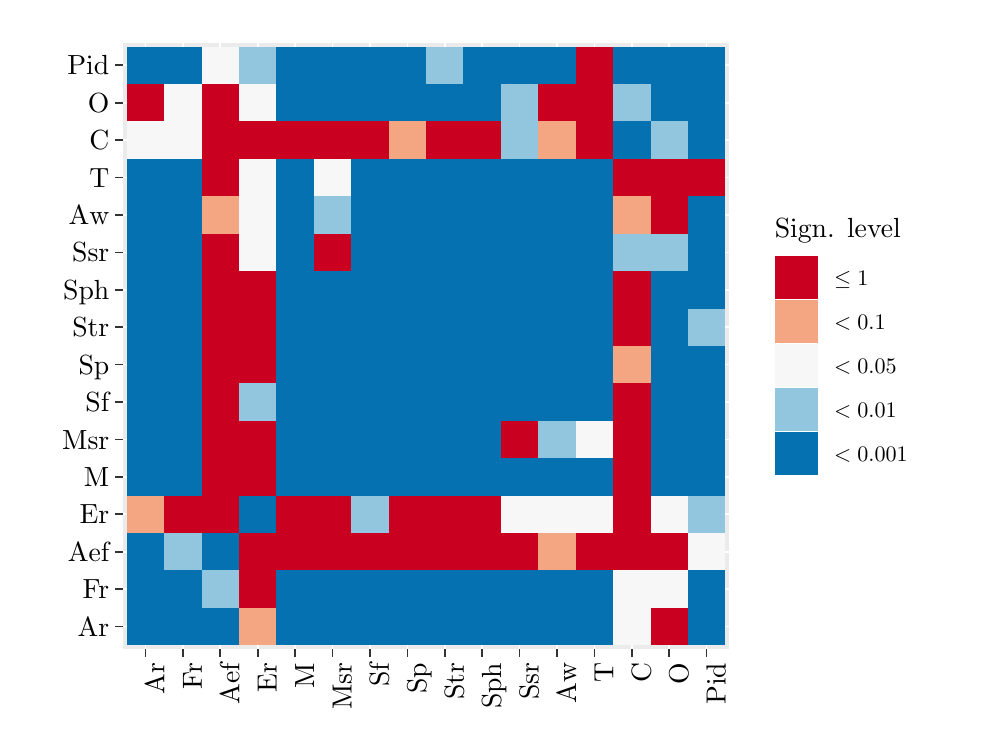
\begin{tikzpicture}[x=1pt,y=1pt]
\definecolor{fillColor}{RGB}{255,255,255}
\path[use as bounding box,fill=fillColor,fill opacity=0.00] (0,0) rectangle (336.00,252.00);
\begin{scope}
\path[clip] (  6.97,  0.00) rectangle (329.03,252.00);
\definecolor{drawColor}{RGB}{255,255,255}
\definecolor{fillColor}{RGB}{255,255,255}

\path[draw=drawColor,line width= 0.6pt,line join=round,line cap=round,fill=fillColor] (  6.97,  0.00) rectangle (329.03,252.00);
\end{scope}
\begin{scope}
\path[clip] ( 34.44, 27.47) rectangle (253.47,246.50);
\definecolor{fillColor}{gray}{0.92}

\path[fill=fillColor] ( 34.44, 27.47) rectangle (253.47,246.50);
\definecolor{drawColor}{RGB}{255,255,255}

\path[draw=drawColor,line width= 0.6pt,line join=round] ( 34.44, 35.59) --
	(253.47, 35.59);

\path[draw=drawColor,line width= 0.6pt,line join=round] ( 34.44, 49.11) --
	(253.47, 49.11);

\path[draw=drawColor,line width= 0.6pt,line join=round] ( 34.44, 62.63) --
	(253.47, 62.63);

\path[draw=drawColor,line width= 0.6pt,line join=round] ( 34.44, 76.15) --
	(253.47, 76.15);

\path[draw=drawColor,line width= 0.6pt,line join=round] ( 34.44, 89.67) --
	(253.47, 89.67);

\path[draw=drawColor,line width= 0.6pt,line join=round] ( 34.44,103.19) --
	(253.47,103.19);

\path[draw=drawColor,line width= 0.6pt,line join=round] ( 34.44,116.71) --
	(253.47,116.71);

\path[draw=drawColor,line width= 0.6pt,line join=round] ( 34.44,130.23) --
	(253.47,130.23);

\path[draw=drawColor,line width= 0.6pt,line join=round] ( 34.44,143.75) --
	(253.47,143.75);

\path[draw=drawColor,line width= 0.6pt,line join=round] ( 34.44,157.27) --
	(253.47,157.27);

\path[draw=drawColor,line width= 0.6pt,line join=round] ( 34.44,170.79) --
	(253.47,170.79);

\path[draw=drawColor,line width= 0.6pt,line join=round] ( 34.44,184.31) --
	(253.47,184.31);

\path[draw=drawColor,line width= 0.6pt,line join=round] ( 34.44,197.83) --
	(253.47,197.83);

\path[draw=drawColor,line width= 0.6pt,line join=round] ( 34.44,211.35) --
	(253.47,211.35);

\path[draw=drawColor,line width= 0.6pt,line join=round] ( 34.44,224.87) --
	(253.47,224.87);

\path[draw=drawColor,line width= 0.6pt,line join=round] ( 34.44,238.39) --
	(253.47,238.39);

\path[draw=drawColor,line width= 0.6pt,line join=round] ( 42.55, 27.47) --
	( 42.55,246.50);

\path[draw=drawColor,line width= 0.6pt,line join=round] ( 56.07, 27.47) --
	( 56.07,246.50);

\path[draw=drawColor,line width= 0.6pt,line join=round] ( 69.59, 27.47) --
	( 69.59,246.50);

\path[draw=drawColor,line width= 0.6pt,line join=round] ( 83.11, 27.47) --
	( 83.11,246.50);

\path[draw=drawColor,line width= 0.6pt,line join=round] ( 96.63, 27.47) --
	( 96.63,246.50);

\path[draw=drawColor,line width= 0.6pt,line join=round] (110.15, 27.47) --
	(110.15,246.50);

\path[draw=drawColor,line width= 0.6pt,line join=round] (123.67, 27.47) --
	(123.67,246.50);

\path[draw=drawColor,line width= 0.6pt,line join=round] (137.19, 27.47) --
	(137.19,246.50);

\path[draw=drawColor,line width= 0.6pt,line join=round] (150.71, 27.47) --
	(150.71,246.50);

\path[draw=drawColor,line width= 0.6pt,line join=round] (164.23, 27.47) --
	(164.23,246.50);

\path[draw=drawColor,line width= 0.6pt,line join=round] (177.75, 27.47) --
	(177.75,246.50);

\path[draw=drawColor,line width= 0.6pt,line join=round] (191.27, 27.47) --
	(191.27,246.50);

\path[draw=drawColor,line width= 0.6pt,line join=round] (204.79, 27.47) --
	(204.79,246.50);

\path[draw=drawColor,line width= 0.6pt,line join=round] (218.31, 27.47) --
	(218.31,246.50);

\path[draw=drawColor,line width= 0.6pt,line join=round] (231.83, 27.47) --
	(231.83,246.50);

\path[draw=drawColor,line width= 0.6pt,line join=round] (245.35, 27.47) --
	(245.35,246.50);
\definecolor{fillColor}{RGB}{5,113,176}

\path[fill=fillColor] ( 35.79, 28.83) rectangle ( 49.31, 42.35);

\path[fill=fillColor] ( 49.31, 28.83) rectangle ( 62.83, 42.35);

\path[fill=fillColor] ( 62.83, 28.83) rectangle ( 76.35, 42.35);
\definecolor{fillColor}{RGB}{244,165,130}

\path[fill=fillColor] ( 76.35, 28.83) rectangle ( 89.87, 42.35);
\definecolor{fillColor}{RGB}{5,113,176}

\path[fill=fillColor] ( 89.87, 28.83) rectangle (103.39, 42.35);

\path[fill=fillColor] (103.39, 28.83) rectangle (116.91, 42.35);

\path[fill=fillColor] (116.91, 28.83) rectangle (130.43, 42.35);

\path[fill=fillColor] (130.43, 28.83) rectangle (143.95, 42.35);

\path[fill=fillColor] (143.95, 28.83) rectangle (157.47, 42.35);

\path[fill=fillColor] (157.47, 28.83) rectangle (170.99, 42.35);

\path[fill=fillColor] (170.99, 28.83) rectangle (184.51, 42.35);

\path[fill=fillColor] (184.51, 28.83) rectangle (198.03, 42.35);

\path[fill=fillColor] (198.03, 28.83) rectangle (211.55, 42.35);
\definecolor{fillColor}{gray}{0.97}

\path[fill=fillColor] (211.55, 28.83) rectangle (225.07, 42.35);
\definecolor{fillColor}{RGB}{202,0,32}

\path[fill=fillColor] (225.07, 28.83) rectangle (238.59, 42.35);
\definecolor{fillColor}{RGB}{5,113,176}

\path[fill=fillColor] (238.59, 28.83) rectangle (252.11, 42.35);

\path[fill=fillColor] ( 35.79, 42.35) rectangle ( 49.31, 55.87);

\path[fill=fillColor] ( 49.31, 42.35) rectangle ( 62.83, 55.87);
\definecolor{fillColor}{RGB}{146,197,222}

\path[fill=fillColor] ( 62.83, 42.35) rectangle ( 76.35, 55.87);
\definecolor{fillColor}{RGB}{202,0,32}

\path[fill=fillColor] ( 76.35, 42.35) rectangle ( 89.87, 55.87);
\definecolor{fillColor}{RGB}{5,113,176}

\path[fill=fillColor] ( 89.87, 42.35) rectangle (103.39, 55.87);

\path[fill=fillColor] (103.39, 42.35) rectangle (116.91, 55.87);

\path[fill=fillColor] (116.91, 42.35) rectangle (130.43, 55.87);

\path[fill=fillColor] (130.43, 42.35) rectangle (143.95, 55.87);

\path[fill=fillColor] (143.95, 42.35) rectangle (157.47, 55.87);

\path[fill=fillColor] (157.47, 42.35) rectangle (170.99, 55.87);

\path[fill=fillColor] (170.99, 42.35) rectangle (184.51, 55.87);

\path[fill=fillColor] (184.51, 42.35) rectangle (198.03, 55.87);

\path[fill=fillColor] (198.03, 42.35) rectangle (211.55, 55.87);
\definecolor{fillColor}{gray}{0.97}

\path[fill=fillColor] (211.55, 42.35) rectangle (225.07, 55.87);

\path[fill=fillColor] (225.07, 42.35) rectangle (238.59, 55.87);
\definecolor{fillColor}{RGB}{5,113,176}

\path[fill=fillColor] (238.59, 42.35) rectangle (252.11, 55.87);

\path[fill=fillColor] ( 35.79, 55.87) rectangle ( 49.31, 69.39);
\definecolor{fillColor}{RGB}{146,197,222}

\path[fill=fillColor] ( 49.31, 55.87) rectangle ( 62.83, 69.39);
\definecolor{fillColor}{RGB}{5,113,176}

\path[fill=fillColor] ( 62.83, 55.87) rectangle ( 76.35, 69.39);
\definecolor{fillColor}{RGB}{202,0,32}

\path[fill=fillColor] ( 76.35, 55.87) rectangle ( 89.87, 69.39);

\path[fill=fillColor] ( 89.87, 55.87) rectangle (103.39, 69.39);

\path[fill=fillColor] (103.39, 55.87) rectangle (116.91, 69.39);

\path[fill=fillColor] (116.91, 55.87) rectangle (130.43, 69.39);

\path[fill=fillColor] (130.43, 55.87) rectangle (143.95, 69.39);

\path[fill=fillColor] (143.95, 55.87) rectangle (157.47, 69.39);

\path[fill=fillColor] (157.47, 55.87) rectangle (170.99, 69.39);

\path[fill=fillColor] (170.99, 55.87) rectangle (184.51, 69.39);
\definecolor{fillColor}{RGB}{244,165,130}

\path[fill=fillColor] (184.51, 55.87) rectangle (198.03, 69.39);
\definecolor{fillColor}{RGB}{202,0,32}

\path[fill=fillColor] (198.03, 55.87) rectangle (211.55, 69.39);

\path[fill=fillColor] (211.55, 55.87) rectangle (225.07, 69.39);

\path[fill=fillColor] (225.07, 55.87) rectangle (238.59, 69.39);
\definecolor{fillColor}{gray}{0.97}

\path[fill=fillColor] (238.59, 55.87) rectangle (252.11, 69.39);
\definecolor{fillColor}{RGB}{244,165,130}

\path[fill=fillColor] ( 35.79, 69.39) rectangle ( 49.31, 82.91);
\definecolor{fillColor}{RGB}{202,0,32}

\path[fill=fillColor] ( 49.31, 69.39) rectangle ( 62.83, 82.91);

\path[fill=fillColor] ( 62.83, 69.39) rectangle ( 76.35, 82.91);
\definecolor{fillColor}{RGB}{5,113,176}

\path[fill=fillColor] ( 76.35, 69.39) rectangle ( 89.87, 82.91);
\definecolor{fillColor}{RGB}{202,0,32}

\path[fill=fillColor] ( 89.87, 69.39) rectangle (103.39, 82.91);

\path[fill=fillColor] (103.39, 69.39) rectangle (116.91, 82.91);
\definecolor{fillColor}{RGB}{146,197,222}

\path[fill=fillColor] (116.91, 69.39) rectangle (130.43, 82.91);
\definecolor{fillColor}{RGB}{202,0,32}

\path[fill=fillColor] (130.43, 69.39) rectangle (143.95, 82.91);

\path[fill=fillColor] (143.95, 69.39) rectangle (157.47, 82.91);

\path[fill=fillColor] (157.47, 69.39) rectangle (170.99, 82.91);
\definecolor{fillColor}{gray}{0.97}

\path[fill=fillColor] (170.99, 69.39) rectangle (184.51, 82.91);

\path[fill=fillColor] (184.51, 69.39) rectangle (198.03, 82.91);

\path[fill=fillColor] (198.03, 69.39) rectangle (211.55, 82.91);
\definecolor{fillColor}{RGB}{202,0,32}

\path[fill=fillColor] (211.55, 69.39) rectangle (225.07, 82.91);
\definecolor{fillColor}{gray}{0.97}

\path[fill=fillColor] (225.07, 69.39) rectangle (238.59, 82.91);
\definecolor{fillColor}{RGB}{146,197,222}

\path[fill=fillColor] (238.59, 69.39) rectangle (252.11, 82.91);
\definecolor{fillColor}{RGB}{5,113,176}

\path[fill=fillColor] ( 35.79, 82.91) rectangle ( 49.31, 96.43);

\path[fill=fillColor] ( 49.31, 82.91) rectangle ( 62.83, 96.43);
\definecolor{fillColor}{RGB}{202,0,32}

\path[fill=fillColor] ( 62.83, 82.91) rectangle ( 76.35, 96.43);

\path[fill=fillColor] ( 76.35, 82.91) rectangle ( 89.87, 96.43);
\definecolor{fillColor}{RGB}{5,113,176}

\path[fill=fillColor] ( 89.87, 82.91) rectangle (103.39, 96.43);

\path[fill=fillColor] (103.39, 82.91) rectangle (116.91, 96.43);

\path[fill=fillColor] (116.91, 82.91) rectangle (130.43, 96.43);

\path[fill=fillColor] (130.43, 82.91) rectangle (143.95, 96.43);

\path[fill=fillColor] (143.95, 82.91) rectangle (157.47, 96.43);

\path[fill=fillColor] (157.47, 82.91) rectangle (170.99, 96.43);

\path[fill=fillColor] (170.99, 82.91) rectangle (184.51, 96.43);

\path[fill=fillColor] (184.51, 82.91) rectangle (198.03, 96.43);

\path[fill=fillColor] (198.03, 82.91) rectangle (211.55, 96.43);
\definecolor{fillColor}{RGB}{202,0,32}

\path[fill=fillColor] (211.55, 82.91) rectangle (225.07, 96.43);
\definecolor{fillColor}{RGB}{5,113,176}

\path[fill=fillColor] (225.07, 82.91) rectangle (238.59, 96.43);

\path[fill=fillColor] (238.59, 82.91) rectangle (252.11, 96.43);

\path[fill=fillColor] ( 35.79, 96.43) rectangle ( 49.31,109.95);

\path[fill=fillColor] ( 49.31, 96.43) rectangle ( 62.83,109.95);
\definecolor{fillColor}{RGB}{202,0,32}

\path[fill=fillColor] ( 62.83, 96.43) rectangle ( 76.35,109.95);

\path[fill=fillColor] ( 76.35, 96.43) rectangle ( 89.87,109.95);
\definecolor{fillColor}{RGB}{5,113,176}

\path[fill=fillColor] ( 89.87, 96.43) rectangle (103.39,109.95);

\path[fill=fillColor] (103.39, 96.43) rectangle (116.91,109.95);

\path[fill=fillColor] (116.91, 96.43) rectangle (130.43,109.95);

\path[fill=fillColor] (130.43, 96.43) rectangle (143.95,109.95);

\path[fill=fillColor] (143.95, 96.43) rectangle (157.47,109.95);

\path[fill=fillColor] (157.47, 96.43) rectangle (170.99,109.95);
\definecolor{fillColor}{RGB}{202,0,32}

\path[fill=fillColor] (170.99, 96.43) rectangle (184.51,109.95);
\definecolor{fillColor}{RGB}{146,197,222}

\path[fill=fillColor] (184.51, 96.43) rectangle (198.03,109.95);
\definecolor{fillColor}{gray}{0.97}

\path[fill=fillColor] (198.03, 96.43) rectangle (211.55,109.95);
\definecolor{fillColor}{RGB}{202,0,32}

\path[fill=fillColor] (211.55, 96.43) rectangle (225.07,109.95);
\definecolor{fillColor}{RGB}{5,113,176}

\path[fill=fillColor] (225.07, 96.43) rectangle (238.59,109.95);

\path[fill=fillColor] (238.59, 96.43) rectangle (252.11,109.95);

\path[fill=fillColor] ( 35.79,109.95) rectangle ( 49.31,123.47);

\path[fill=fillColor] ( 49.31,109.95) rectangle ( 62.83,123.47);
\definecolor{fillColor}{RGB}{202,0,32}

\path[fill=fillColor] ( 62.83,109.95) rectangle ( 76.35,123.47);
\definecolor{fillColor}{RGB}{146,197,222}

\path[fill=fillColor] ( 76.35,109.95) rectangle ( 89.87,123.47);
\definecolor{fillColor}{RGB}{5,113,176}

\path[fill=fillColor] ( 89.87,109.95) rectangle (103.39,123.47);

\path[fill=fillColor] (103.39,109.95) rectangle (116.91,123.47);

\path[fill=fillColor] (116.91,109.95) rectangle (130.43,123.47);

\path[fill=fillColor] (130.43,109.95) rectangle (143.95,123.47);

\path[fill=fillColor] (143.95,109.95) rectangle (157.47,123.47);

\path[fill=fillColor] (157.47,109.95) rectangle (170.99,123.47);

\path[fill=fillColor] (170.99,109.95) rectangle (184.51,123.47);

\path[fill=fillColor] (184.51,109.95) rectangle (198.03,123.47);

\path[fill=fillColor] (198.03,109.95) rectangle (211.55,123.47);
\definecolor{fillColor}{RGB}{202,0,32}

\path[fill=fillColor] (211.55,109.95) rectangle (225.07,123.47);
\definecolor{fillColor}{RGB}{5,113,176}

\path[fill=fillColor] (225.07,109.95) rectangle (238.59,123.47);

\path[fill=fillColor] (238.59,109.95) rectangle (252.11,123.47);

\path[fill=fillColor] ( 35.79,123.47) rectangle ( 49.31,136.99);

\path[fill=fillColor] ( 49.31,123.47) rectangle ( 62.83,136.99);
\definecolor{fillColor}{RGB}{202,0,32}

\path[fill=fillColor] ( 62.83,123.47) rectangle ( 76.35,136.99);

\path[fill=fillColor] ( 76.35,123.47) rectangle ( 89.87,136.99);
\definecolor{fillColor}{RGB}{5,113,176}

\path[fill=fillColor] ( 89.87,123.47) rectangle (103.39,136.99);

\path[fill=fillColor] (103.39,123.47) rectangle (116.91,136.99);

\path[fill=fillColor] (116.91,123.47) rectangle (130.43,136.99);

\path[fill=fillColor] (130.43,123.47) rectangle (143.95,136.99);

\path[fill=fillColor] (143.95,123.47) rectangle (157.47,136.99);

\path[fill=fillColor] (157.47,123.47) rectangle (170.99,136.99);

\path[fill=fillColor] (170.99,123.47) rectangle (184.51,136.99);

\path[fill=fillColor] (184.51,123.47) rectangle (198.03,136.99);

\path[fill=fillColor] (198.03,123.47) rectangle (211.55,136.99);
\definecolor{fillColor}{RGB}{244,165,130}

\path[fill=fillColor] (211.55,123.47) rectangle (225.07,136.99);
\definecolor{fillColor}{RGB}{5,113,176}

\path[fill=fillColor] (225.07,123.47) rectangle (238.59,136.99);

\path[fill=fillColor] (238.59,123.47) rectangle (252.11,136.99);

\path[fill=fillColor] ( 35.79,136.99) rectangle ( 49.31,150.51);

\path[fill=fillColor] ( 49.31,136.99) rectangle ( 62.83,150.51);
\definecolor{fillColor}{RGB}{202,0,32}

\path[fill=fillColor] ( 62.83,136.99) rectangle ( 76.35,150.51);

\path[fill=fillColor] ( 76.35,136.99) rectangle ( 89.87,150.51);
\definecolor{fillColor}{RGB}{5,113,176}

\path[fill=fillColor] ( 89.87,136.99) rectangle (103.39,150.51);

\path[fill=fillColor] (103.39,136.99) rectangle (116.91,150.51);

\path[fill=fillColor] (116.91,136.99) rectangle (130.43,150.51);

\path[fill=fillColor] (130.43,136.99) rectangle (143.95,150.51);

\path[fill=fillColor] (143.95,136.99) rectangle (157.47,150.51);

\path[fill=fillColor] (157.47,136.99) rectangle (170.99,150.51);

\path[fill=fillColor] (170.99,136.99) rectangle (184.51,150.51);

\path[fill=fillColor] (184.51,136.99) rectangle (198.03,150.51);

\path[fill=fillColor] (198.03,136.99) rectangle (211.55,150.51);
\definecolor{fillColor}{RGB}{202,0,32}

\path[fill=fillColor] (211.55,136.99) rectangle (225.07,150.51);
\definecolor{fillColor}{RGB}{5,113,176}

\path[fill=fillColor] (225.07,136.99) rectangle (238.59,150.51);
\definecolor{fillColor}{RGB}{146,197,222}

\path[fill=fillColor] (238.59,136.99) rectangle (252.11,150.51);
\definecolor{fillColor}{RGB}{5,113,176}

\path[fill=fillColor] ( 35.79,150.51) rectangle ( 49.31,164.03);

\path[fill=fillColor] ( 49.31,150.51) rectangle ( 62.83,164.03);
\definecolor{fillColor}{RGB}{202,0,32}

\path[fill=fillColor] ( 62.83,150.51) rectangle ( 76.35,164.03);

\path[fill=fillColor] ( 76.35,150.51) rectangle ( 89.87,164.03);
\definecolor{fillColor}{RGB}{5,113,176}

\path[fill=fillColor] ( 89.87,150.51) rectangle (103.39,164.03);

\path[fill=fillColor] (103.39,150.51) rectangle (116.91,164.03);

\path[fill=fillColor] (116.91,150.51) rectangle (130.43,164.03);

\path[fill=fillColor] (130.43,150.51) rectangle (143.95,164.03);

\path[fill=fillColor] (143.95,150.51) rectangle (157.47,164.03);

\path[fill=fillColor] (157.47,150.51) rectangle (170.99,164.03);

\path[fill=fillColor] (170.99,150.51) rectangle (184.51,164.03);

\path[fill=fillColor] (184.51,150.51) rectangle (198.03,164.03);

\path[fill=fillColor] (198.03,150.51) rectangle (211.55,164.03);
\definecolor{fillColor}{RGB}{202,0,32}

\path[fill=fillColor] (211.55,150.51) rectangle (225.07,164.03);
\definecolor{fillColor}{RGB}{5,113,176}

\path[fill=fillColor] (225.07,150.51) rectangle (238.59,164.03);

\path[fill=fillColor] (238.59,150.51) rectangle (252.11,164.03);

\path[fill=fillColor] ( 35.79,164.03) rectangle ( 49.31,177.55);

\path[fill=fillColor] ( 49.31,164.03) rectangle ( 62.83,177.55);
\definecolor{fillColor}{RGB}{202,0,32}

\path[fill=fillColor] ( 62.83,164.03) rectangle ( 76.35,177.55);
\definecolor{fillColor}{gray}{0.97}

\path[fill=fillColor] ( 76.35,164.03) rectangle ( 89.87,177.55);
\definecolor{fillColor}{RGB}{5,113,176}

\path[fill=fillColor] ( 89.87,164.03) rectangle (103.39,177.55);
\definecolor{fillColor}{RGB}{202,0,32}

\path[fill=fillColor] (103.39,164.03) rectangle (116.91,177.55);
\definecolor{fillColor}{RGB}{5,113,176}

\path[fill=fillColor] (116.91,164.03) rectangle (130.43,177.55);

\path[fill=fillColor] (130.43,164.03) rectangle (143.95,177.55);

\path[fill=fillColor] (143.95,164.03) rectangle (157.47,177.55);

\path[fill=fillColor] (157.47,164.03) rectangle (170.99,177.55);

\path[fill=fillColor] (170.99,164.03) rectangle (184.51,177.55);

\path[fill=fillColor] (184.51,164.03) rectangle (198.03,177.55);

\path[fill=fillColor] (198.03,164.03) rectangle (211.55,177.55);
\definecolor{fillColor}{RGB}{146,197,222}

\path[fill=fillColor] (211.55,164.03) rectangle (225.07,177.55);

\path[fill=fillColor] (225.07,164.03) rectangle (238.59,177.55);
\definecolor{fillColor}{RGB}{5,113,176}

\path[fill=fillColor] (238.59,164.03) rectangle (252.11,177.55);

\path[fill=fillColor] ( 35.79,177.55) rectangle ( 49.31,191.07);

\path[fill=fillColor] ( 49.31,177.55) rectangle ( 62.83,191.07);
\definecolor{fillColor}{RGB}{244,165,130}

\path[fill=fillColor] ( 62.83,177.55) rectangle ( 76.35,191.07);
\definecolor{fillColor}{gray}{0.97}

\path[fill=fillColor] ( 76.35,177.55) rectangle ( 89.87,191.07);
\definecolor{fillColor}{RGB}{5,113,176}

\path[fill=fillColor] ( 89.87,177.55) rectangle (103.39,191.07);
\definecolor{fillColor}{RGB}{146,197,222}

\path[fill=fillColor] (103.39,177.55) rectangle (116.91,191.07);
\definecolor{fillColor}{RGB}{5,113,176}

\path[fill=fillColor] (116.91,177.55) rectangle (130.43,191.07);

\path[fill=fillColor] (130.43,177.55) rectangle (143.95,191.07);

\path[fill=fillColor] (143.95,177.55) rectangle (157.47,191.07);

\path[fill=fillColor] (157.47,177.55) rectangle (170.99,191.07);

\path[fill=fillColor] (170.99,177.55) rectangle (184.51,191.07);

\path[fill=fillColor] (184.51,177.55) rectangle (198.03,191.07);

\path[fill=fillColor] (198.03,177.55) rectangle (211.55,191.07);
\definecolor{fillColor}{RGB}{244,165,130}

\path[fill=fillColor] (211.55,177.55) rectangle (225.07,191.07);
\definecolor{fillColor}{RGB}{202,0,32}

\path[fill=fillColor] (225.07,177.55) rectangle (238.59,191.07);
\definecolor{fillColor}{RGB}{5,113,176}

\path[fill=fillColor] (238.59,177.55) rectangle (252.11,191.07);

\path[fill=fillColor] ( 35.79,191.07) rectangle ( 49.31,204.59);

\path[fill=fillColor] ( 49.31,191.07) rectangle ( 62.83,204.59);
\definecolor{fillColor}{RGB}{202,0,32}

\path[fill=fillColor] ( 62.83,191.07) rectangle ( 76.35,204.59);
\definecolor{fillColor}{gray}{0.97}

\path[fill=fillColor] ( 76.35,191.07) rectangle ( 89.87,204.59);
\definecolor{fillColor}{RGB}{5,113,176}

\path[fill=fillColor] ( 89.87,191.07) rectangle (103.39,204.59);
\definecolor{fillColor}{gray}{0.97}

\path[fill=fillColor] (103.39,191.07) rectangle (116.91,204.59);
\definecolor{fillColor}{RGB}{5,113,176}

\path[fill=fillColor] (116.91,191.07) rectangle (130.43,204.59);

\path[fill=fillColor] (130.43,191.07) rectangle (143.95,204.59);

\path[fill=fillColor] (143.95,191.07) rectangle (157.47,204.59);

\path[fill=fillColor] (157.47,191.07) rectangle (170.99,204.59);

\path[fill=fillColor] (170.99,191.07) rectangle (184.51,204.59);

\path[fill=fillColor] (184.51,191.07) rectangle (198.03,204.59);

\path[fill=fillColor] (198.03,191.07) rectangle (211.55,204.59);
\definecolor{fillColor}{RGB}{202,0,32}

\path[fill=fillColor] (211.55,191.07) rectangle (225.07,204.59);

\path[fill=fillColor] (225.07,191.07) rectangle (238.59,204.59);

\path[fill=fillColor] (238.59,191.07) rectangle (252.11,204.59);
\definecolor{fillColor}{gray}{0.97}

\path[fill=fillColor] ( 35.79,204.59) rectangle ( 49.31,218.11);

\path[fill=fillColor] ( 49.31,204.59) rectangle ( 62.83,218.11);
\definecolor{fillColor}{RGB}{202,0,32}

\path[fill=fillColor] ( 62.83,204.59) rectangle ( 76.35,218.11);

\path[fill=fillColor] ( 76.35,204.59) rectangle ( 89.87,218.11);

\path[fill=fillColor] ( 89.87,204.59) rectangle (103.39,218.11);

\path[fill=fillColor] (103.39,204.59) rectangle (116.91,218.11);

\path[fill=fillColor] (116.91,204.59) rectangle (130.43,218.11);
\definecolor{fillColor}{RGB}{244,165,130}

\path[fill=fillColor] (130.43,204.59) rectangle (143.95,218.11);
\definecolor{fillColor}{RGB}{202,0,32}

\path[fill=fillColor] (143.95,204.59) rectangle (157.47,218.11);

\path[fill=fillColor] (157.47,204.59) rectangle (170.99,218.11);
\definecolor{fillColor}{RGB}{146,197,222}

\path[fill=fillColor] (170.99,204.59) rectangle (184.51,218.11);
\definecolor{fillColor}{RGB}{244,165,130}

\path[fill=fillColor] (184.51,204.59) rectangle (198.03,218.11);
\definecolor{fillColor}{RGB}{202,0,32}

\path[fill=fillColor] (198.03,204.59) rectangle (211.55,218.11);
\definecolor{fillColor}{RGB}{5,113,176}

\path[fill=fillColor] (211.55,204.59) rectangle (225.07,218.11);
\definecolor{fillColor}{RGB}{146,197,222}

\path[fill=fillColor] (225.07,204.59) rectangle (238.59,218.11);
\definecolor{fillColor}{RGB}{5,113,176}

\path[fill=fillColor] (238.59,204.59) rectangle (252.11,218.11);
\definecolor{fillColor}{RGB}{202,0,32}

\path[fill=fillColor] ( 35.79,218.11) rectangle ( 49.31,231.63);
\definecolor{fillColor}{gray}{0.97}

\path[fill=fillColor] ( 49.31,218.11) rectangle ( 62.83,231.63);
\definecolor{fillColor}{RGB}{202,0,32}

\path[fill=fillColor] ( 62.83,218.11) rectangle ( 76.35,231.63);
\definecolor{fillColor}{gray}{0.97}

\path[fill=fillColor] ( 76.35,218.11) rectangle ( 89.87,231.63);
\definecolor{fillColor}{RGB}{5,113,176}

\path[fill=fillColor] ( 89.87,218.11) rectangle (103.39,231.63);

\path[fill=fillColor] (103.39,218.11) rectangle (116.91,231.63);

\path[fill=fillColor] (116.91,218.11) rectangle (130.43,231.63);

\path[fill=fillColor] (130.43,218.11) rectangle (143.95,231.63);

\path[fill=fillColor] (143.95,218.11) rectangle (157.47,231.63);

\path[fill=fillColor] (157.47,218.11) rectangle (170.99,231.63);
\definecolor{fillColor}{RGB}{146,197,222}

\path[fill=fillColor] (170.99,218.11) rectangle (184.51,231.63);
\definecolor{fillColor}{RGB}{202,0,32}

\path[fill=fillColor] (184.51,218.11) rectangle (198.03,231.63);

\path[fill=fillColor] (198.03,218.11) rectangle (211.55,231.63);
\definecolor{fillColor}{RGB}{146,197,222}

\path[fill=fillColor] (211.55,218.11) rectangle (225.07,231.63);
\definecolor{fillColor}{RGB}{5,113,176}

\path[fill=fillColor] (225.07,218.11) rectangle (238.59,231.63);

\path[fill=fillColor] (238.59,218.11) rectangle (252.11,231.63);

\path[fill=fillColor] ( 35.79,231.63) rectangle ( 49.31,245.15);

\path[fill=fillColor] ( 49.31,231.63) rectangle ( 62.83,245.15);
\definecolor{fillColor}{gray}{0.97}

\path[fill=fillColor] ( 62.83,231.63) rectangle ( 76.35,245.15);
\definecolor{fillColor}{RGB}{146,197,222}

\path[fill=fillColor] ( 76.35,231.63) rectangle ( 89.87,245.15);
\definecolor{fillColor}{RGB}{5,113,176}

\path[fill=fillColor] ( 89.87,231.63) rectangle (103.39,245.15);

\path[fill=fillColor] (103.39,231.63) rectangle (116.91,245.15);

\path[fill=fillColor] (116.91,231.63) rectangle (130.43,245.15);

\path[fill=fillColor] (130.43,231.63) rectangle (143.95,245.15);
\definecolor{fillColor}{RGB}{146,197,222}

\path[fill=fillColor] (143.95,231.63) rectangle (157.47,245.15);
\definecolor{fillColor}{RGB}{5,113,176}

\path[fill=fillColor] (157.47,231.63) rectangle (170.99,245.15);

\path[fill=fillColor] (170.99,231.63) rectangle (184.51,245.15);

\path[fill=fillColor] (184.51,231.63) rectangle (198.03,245.15);
\definecolor{fillColor}{RGB}{202,0,32}

\path[fill=fillColor] (198.03,231.63) rectangle (211.55,245.15);
\definecolor{fillColor}{RGB}{5,113,176}

\path[fill=fillColor] (211.55,231.63) rectangle (225.07,245.15);

\path[fill=fillColor] (225.07,231.63) rectangle (238.59,245.15);

\path[fill=fillColor] (238.59,231.63) rectangle (252.11,245.15);
\end{scope}
\begin{scope}
\path[clip] (  0.00,  0.00) rectangle (336.00,252.00);
\definecolor{drawColor}{RGB}{0,0,0}

\node[text=drawColor,anchor=base east,inner sep=0pt, outer sep=0pt, scale=  1.00] at ( 29.49, 32.14) {Ar};

\node[text=drawColor,anchor=base east,inner sep=0pt, outer sep=0pt, scale=  1.00] at ( 29.49, 45.66) {Fr};

\node[text=drawColor,anchor=base east,inner sep=0pt, outer sep=0pt, scale=  1.00] at ( 29.49, 59.18) {Aef};

\node[text=drawColor,anchor=base east,inner sep=0pt, outer sep=0pt, scale=  1.00] at ( 29.49, 72.70) {Er};

\node[text=drawColor,anchor=base east,inner sep=0pt, outer sep=0pt, scale=  1.00] at ( 29.49, 86.22) {M};

\node[text=drawColor,anchor=base east,inner sep=0pt, outer sep=0pt, scale=  1.00] at ( 29.49, 99.74) {Msr};

\node[text=drawColor,anchor=base east,inner sep=0pt, outer sep=0pt, scale=  1.00] at ( 29.49,113.26) {Sf};

\node[text=drawColor,anchor=base east,inner sep=0pt, outer sep=0pt, scale=  1.00] at ( 29.49,126.78) {Sp};

\node[text=drawColor,anchor=base east,inner sep=0pt, outer sep=0pt, scale=  1.00] at ( 29.49,140.30) {Str};

\node[text=drawColor,anchor=base east,inner sep=0pt, outer sep=0pt, scale=  1.00] at ( 29.49,153.82) {Sph};

\node[text=drawColor,anchor=base east,inner sep=0pt, outer sep=0pt, scale=  1.00] at ( 29.49,167.34) {Ssr};

\node[text=drawColor,anchor=base east,inner sep=0pt, outer sep=0pt, scale=  1.00] at ( 29.49,180.86) {Aw};

\node[text=drawColor,anchor=base east,inner sep=0pt, outer sep=0pt, scale=  1.00] at ( 29.49,194.38) {T};

\node[text=drawColor,anchor=base east,inner sep=0pt, outer sep=0pt, scale=  1.00] at ( 29.49,207.90) {C};

\node[text=drawColor,anchor=base east,inner sep=0pt, outer sep=0pt, scale=  1.00] at ( 29.49,221.42) {O};

\node[text=drawColor,anchor=base east,inner sep=0pt, outer sep=0pt, scale=  1.00] at ( 29.49,234.94) {Pid};
\end{scope}
\begin{scope}
\path[clip] (  0.00,  0.00) rectangle (336.00,252.00);
\definecolor{drawColor}{gray}{0.20}

\path[draw=drawColor,line width= 0.6pt,line join=round] ( 31.69, 35.59) --
	( 34.44, 35.59);

\path[draw=drawColor,line width= 0.6pt,line join=round] ( 31.69, 49.11) --
	( 34.44, 49.11);

\path[draw=drawColor,line width= 0.6pt,line join=round] ( 31.69, 62.63) --
	( 34.44, 62.63);

\path[draw=drawColor,line width= 0.6pt,line join=round] ( 31.69, 76.15) --
	( 34.44, 76.15);

\path[draw=drawColor,line width= 0.6pt,line join=round] ( 31.69, 89.67) --
	( 34.44, 89.67);

\path[draw=drawColor,line width= 0.6pt,line join=round] ( 31.69,103.19) --
	( 34.44,103.19);

\path[draw=drawColor,line width= 0.6pt,line join=round] ( 31.69,116.71) --
	( 34.44,116.71);

\path[draw=drawColor,line width= 0.6pt,line join=round] ( 31.69,130.23) --
	( 34.44,130.23);

\path[draw=drawColor,line width= 0.6pt,line join=round] ( 31.69,143.75) --
	( 34.44,143.75);

\path[draw=drawColor,line width= 0.6pt,line join=round] ( 31.69,157.27) --
	( 34.44,157.27);

\path[draw=drawColor,line width= 0.6pt,line join=round] ( 31.69,170.79) --
	( 34.44,170.79);

\path[draw=drawColor,line width= 0.6pt,line join=round] ( 31.69,184.31) --
	( 34.44,184.31);

\path[draw=drawColor,line width= 0.6pt,line join=round] ( 31.69,197.83) --
	( 34.44,197.83);

\path[draw=drawColor,line width= 0.6pt,line join=round] ( 31.69,211.35) --
	( 34.44,211.35);

\path[draw=drawColor,line width= 0.6pt,line join=round] ( 31.69,224.87) --
	( 34.44,224.87);

\path[draw=drawColor,line width= 0.6pt,line join=round] ( 31.69,238.39) --
	( 34.44,238.39);
\end{scope}
\begin{scope}
\path[clip] (  0.00,  0.00) rectangle (336.00,252.00);
\definecolor{drawColor}{gray}{0.20}

\path[draw=drawColor,line width= 0.6pt,line join=round] ( 42.55, 24.72) --
	( 42.55, 27.47);

\path[draw=drawColor,line width= 0.6pt,line join=round] ( 56.07, 24.72) --
	( 56.07, 27.47);

\path[draw=drawColor,line width= 0.6pt,line join=round] ( 69.59, 24.72) --
	( 69.59, 27.47);

\path[draw=drawColor,line width= 0.6pt,line join=round] ( 83.11, 24.72) --
	( 83.11, 27.47);

\path[draw=drawColor,line width= 0.6pt,line join=round] ( 96.63, 24.72) --
	( 96.63, 27.47);

\path[draw=drawColor,line width= 0.6pt,line join=round] (110.15, 24.72) --
	(110.15, 27.47);

\path[draw=drawColor,line width= 0.6pt,line join=round] (123.67, 24.72) --
	(123.67, 27.47);

\path[draw=drawColor,line width= 0.6pt,line join=round] (137.19, 24.72) --
	(137.19, 27.47);

\path[draw=drawColor,line width= 0.6pt,line join=round] (150.71, 24.72) --
	(150.71, 27.47);

\path[draw=drawColor,line width= 0.6pt,line join=round] (164.23, 24.72) --
	(164.23, 27.47);

\path[draw=drawColor,line width= 0.6pt,line join=round] (177.75, 24.72) --
	(177.75, 27.47);

\path[draw=drawColor,line width= 0.6pt,line join=round] (191.27, 24.72) --
	(191.27, 27.47);

\path[draw=drawColor,line width= 0.6pt,line join=round] (204.79, 24.72) --
	(204.79, 27.47);

\path[draw=drawColor,line width= 0.6pt,line join=round] (218.31, 24.72) --
	(218.31, 27.47);

\path[draw=drawColor,line width= 0.6pt,line join=round] (231.83, 24.72) --
	(231.83, 27.47);

\path[draw=drawColor,line width= 0.6pt,line join=round] (245.35, 24.72) --
	(245.35, 27.47);
\end{scope}
\begin{scope}
\path[clip] (  0.00,  0.00) rectangle (336.00,252.00);
\definecolor{drawColor}{RGB}{0,0,0}

\node[text=drawColor,rotate= 90.00,anchor=base east,inner sep=0pt, outer sep=0pt, scale=  1.00] at ( 49.44, 22.52) {Ar};

\node[text=drawColor,rotate= 90.00,anchor=base east,inner sep=0pt, outer sep=0pt, scale=  1.00] at ( 62.96, 22.52) {Fr};

\node[text=drawColor,rotate= 90.00,anchor=base east,inner sep=0pt, outer sep=0pt, scale=  1.00] at ( 76.48, 22.52) {Aef};

\node[text=drawColor,rotate= 90.00,anchor=base east,inner sep=0pt, outer sep=0pt, scale=  1.00] at ( 90.00, 22.52) {Er};

\node[text=drawColor,rotate= 90.00,anchor=base east,inner sep=0pt, outer sep=0pt, scale=  1.00] at (103.52, 22.52) {M};

\node[text=drawColor,rotate= 90.00,anchor=base east,inner sep=0pt, outer sep=0pt, scale=  1.00] at (117.04, 22.52) {Msr};

\node[text=drawColor,rotate= 90.00,anchor=base east,inner sep=0pt, outer sep=0pt, scale=  1.00] at (130.56, 22.52) {Sf};

\node[text=drawColor,rotate= 90.00,anchor=base east,inner sep=0pt, outer sep=0pt, scale=  1.00] at (144.08, 22.52) {Sp};

\node[text=drawColor,rotate= 90.00,anchor=base east,inner sep=0pt, outer sep=0pt, scale=  1.00] at (157.60, 22.52) {Str};

\node[text=drawColor,rotate= 90.00,anchor=base east,inner sep=0pt, outer sep=0pt, scale=  1.00] at (171.12, 22.52) {Sph};

\node[text=drawColor,rotate= 90.00,anchor=base east,inner sep=0pt, outer sep=0pt, scale=  1.00] at (184.64, 22.52) {Ssr};

\node[text=drawColor,rotate= 90.00,anchor=base east,inner sep=0pt, outer sep=0pt, scale=  1.00] at (198.16, 22.52) {Aw};

\node[text=drawColor,rotate= 90.00,anchor=base east,inner sep=0pt, outer sep=0pt, scale=  1.00] at (211.68, 22.52) {T};

\node[text=drawColor,rotate= 90.00,anchor=base east,inner sep=0pt, outer sep=0pt, scale=  1.00] at (225.20, 22.52) {C};

\node[text=drawColor,rotate= 90.00,anchor=base east,inner sep=0pt, outer sep=0pt, scale=  1.00] at (238.72, 22.52) {O};

\node[text=drawColor,rotate= 90.00,anchor=base east,inner sep=0pt, outer sep=0pt, scale=  1.00] at (252.24, 22.52) {Pid};
\end{scope}
\begin{scope}
\path[clip] (  0.00,  0.00) rectangle (336.00,252.00);
\definecolor{fillColor}{RGB}{255,255,255}

\path[fill=fillColor] (264.47, 84.57) rectangle (323.53,189.40);
\end{scope}
\begin{scope}
\path[clip] (  0.00,  0.00) rectangle (336.00,252.00);
\definecolor{drawColor}{RGB}{0,0,0}

\node[text=drawColor,anchor=base west,inner sep=0pt, outer sep=0pt, scale=  1.00] at (269.97,176.04) {Sign. level};
\end{scope}
\begin{scope}
\path[clip] (  0.00,  0.00) rectangle (336.00,252.00);
\definecolor{drawColor}{RGB}{255,255,255}
\definecolor{fillColor}{gray}{0.95}

\path[draw=drawColor,line width= 0.6pt,line join=round,line cap=round,fill=fillColor] (269.97,153.67) rectangle (285.87,169.57);
\end{scope}
\begin{scope}
\path[clip] (  0.00,  0.00) rectangle (336.00,252.00);
\definecolor{fillColor}{RGB}{202,0,32}

\path[fill=fillColor] (270.11,153.81) rectangle (285.72,169.43);
\end{scope}
\begin{scope}
\path[clip] (  0.00,  0.00) rectangle (336.00,252.00);
\definecolor{drawColor}{RGB}{255,255,255}
\definecolor{fillColor}{gray}{0.95}

\path[draw=drawColor,line width= 0.6pt,line join=round,line cap=round,fill=fillColor] (269.97,137.77) rectangle (285.87,153.67);
\end{scope}
\begin{scope}
\path[clip] (  0.00,  0.00) rectangle (336.00,252.00);
\definecolor{fillColor}{RGB}{244,165,130}

\path[fill=fillColor] (270.11,137.91) rectangle (285.72,153.53);
\end{scope}
\begin{scope}
\path[clip] (  0.00,  0.00) rectangle (336.00,252.00);
\definecolor{drawColor}{RGB}{255,255,255}
\definecolor{fillColor}{gray}{0.95}

\path[draw=drawColor,line width= 0.6pt,line join=round,line cap=round,fill=fillColor] (269.97,121.87) rectangle (285.87,137.77);
\end{scope}
\begin{scope}
\path[clip] (  0.00,  0.00) rectangle (336.00,252.00);
\definecolor{fillColor}{gray}{0.97}

\path[fill=fillColor] (270.11,122.01) rectangle (285.72,137.63);
\end{scope}
\begin{scope}
\path[clip] (  0.00,  0.00) rectangle (336.00,252.00);
\definecolor{drawColor}{RGB}{255,255,255}
\definecolor{fillColor}{gray}{0.95}

\path[draw=drawColor,line width= 0.6pt,line join=round,line cap=round,fill=fillColor] (269.97,105.97) rectangle (285.87,121.87);
\end{scope}
\begin{scope}
\path[clip] (  0.00,  0.00) rectangle (336.00,252.00);
\definecolor{fillColor}{RGB}{146,197,222}

\path[fill=fillColor] (270.11,106.11) rectangle (285.72,121.73);
\end{scope}
\begin{scope}
\path[clip] (  0.00,  0.00) rectangle (336.00,252.00);
\definecolor{drawColor}{RGB}{255,255,255}
\definecolor{fillColor}{gray}{0.95}

\path[draw=drawColor,line width= 0.6pt,line join=round,line cap=round,fill=fillColor] (269.97, 90.07) rectangle (285.87,105.97);
\end{scope}
\begin{scope}
\path[clip] (  0.00,  0.00) rectangle (336.00,252.00);
\definecolor{fillColor}{RGB}{5,113,176}

\path[fill=fillColor] (270.11, 90.21) rectangle (285.72,105.83);
\end{scope}
\begin{scope}
\path[clip] (  0.00,  0.00) rectangle (336.00,252.00);
\definecolor{drawColor}{RGB}{0,0,0}

\node[text=drawColor,anchor=base west,inner sep=0pt, outer sep=0pt, scale=  0.80] at (291.37,158.87) {\( \leq 1\)};
\end{scope}
\begin{scope}
\path[clip] (  0.00,  0.00) rectangle (336.00,252.00);
\definecolor{drawColor}{RGB}{0,0,0}

\node[text=drawColor,anchor=base west,inner sep=0pt, outer sep=0pt, scale=  0.80] at (291.37,142.97) {\(< 0.1\)};
\end{scope}
\begin{scope}
\path[clip] (  0.00,  0.00) rectangle (336.00,252.00);
\definecolor{drawColor}{RGB}{0,0,0}

\node[text=drawColor,anchor=base west,inner sep=0pt, outer sep=0pt, scale=  0.80] at (291.37,127.07) {\(< 0.05\)};
\end{scope}
\begin{scope}
\path[clip] (  0.00,  0.00) rectangle (336.00,252.00);
\definecolor{drawColor}{RGB}{0,0,0}

\node[text=drawColor,anchor=base west,inner sep=0pt, outer sep=0pt, scale=  0.80] at (291.37,111.17) {\(< 0.01\)};
\end{scope}
\begin{scope}
\path[clip] (  0.00,  0.00) rectangle (336.00,252.00);
\definecolor{drawColor}{RGB}{0,0,0}

\node[text=drawColor,anchor=base west,inner sep=0pt, outer sep=0pt, scale=  0.80] at (291.37, 95.27) {\(< 0.001\)};
\end{scope}
\end{tikzpicture}
